\documentclass[letterpaper]{article}
\usepackage{natbib,alifexi}
\usepackage[utf8]{inputenc}
\usepackage[frenchb]{babel}
\usepackage{comment}

\title{Time stretching en temps réel pour le live coding}
\author{Abdeselam El-Haman Abdeselam$^{1}$\\
Superviseur : Bernard Fortz
\mbox{}\\\\
$^1$Université Libre de Bruxelles \\
aelhaman@ulb.ac.be}


\begin{document}
\maketitle

\begin{abstract}
  Overtone est une libraire en Clojure qui est utilisée pour faire du
  Live Coding (l'art de programmer en \og vif \fg{}). Une des techniques les
  plus utilisées dans le domaine de la musique synthétisée est le
  time-stretching, qui consiste à rallonger ou rétrécir une pièce musicale
  sans changer sa tonalité. Le time-stretching est intéressant dans
  le live-coding lorsqu'on peut modifier les paramétres de celui-ci
  en temps réel. Dans cet article 2 méthodes de time-stretching avec des
  approches différentes seront analysées, comparées et utilisées en temps
  réel dans Overtone.

\end{abstract}

\section{Introduction}

  Depuis le débuts de la musique éléctronique, le ``resampling'' de pièces musicales
  (c'est à dire, la manipulation de celles-ci) a un rôle important pour pouvoir manipuler
  des pièces musicales (rajouter des filtres, des envelopes, etc...) [rajouter citation ici].

  Une de ces techniques est la manipulation de la pièce dans le temps, en changeant sa durée
  en

  Le time-stretching est une technique qui consiste en rallonger ou
  rétrécir 

  \begin{figure}[h]
    \centerline{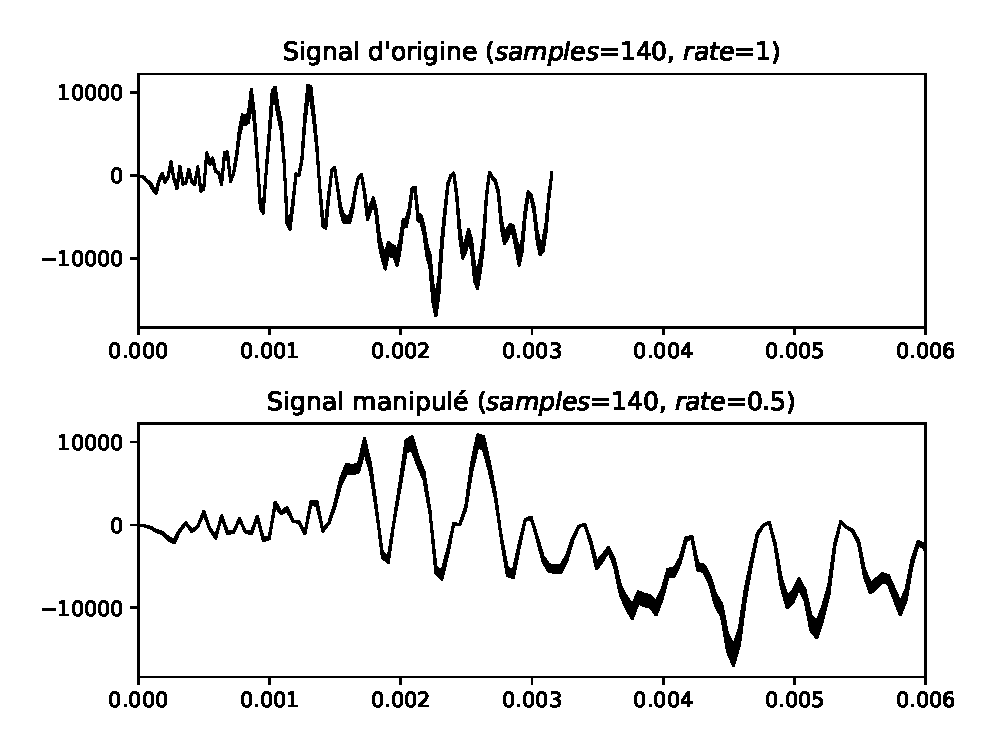
\includegraphics[width=9cm]{res/fig1.eps}}
    \caption{\label{fig:guitar-stretch}Sample d'une guitare lu à des ratios différents}
  \end{figure}
  
  Le time-stretching est une technique qui consiste en rallonger ou
  rétrécir synth


 
\begin{comment}
  Parler du son c'est quoi frequence etc

  C'est quoi le problème time stretching?
  À quoi est-il dû?
\end{comment}

\section{État de l'art}
\begin{comment}
  Techniques, un peu d'histoire?
\end{comment}

\subsection{Traitement du temps}
\begin{comment}
Parler de SOLA, PSOLA...
\end{comment}

\subsection{Traitement des fréquences}
\begin{comment}
  Parler du Vocodeur de phases, comment c'est utilisé etc...
\end{comment}
\subsection{Traitement du temps et des fréquences}
\begin{comment}
  On parle des techniques comme PVSOLA -> SOLA en prenant en compte la phase etc
\end{comment}

\section{Méthodes}

Les 2 méthodes qui ont été développées sont la granulation et le vocodeur de phases.
Ces 2 méthodes ont été utilisées en utilisant la fonction le système de génération de
synthétiseurs ``defsynth'' d'Overtone.
\begin{comment}
  Parler d'Overtone, Supercollider...
  UGENs qu'on va utiliser: PVRecordBuf, PVPlayBuf..
\end{comment}

\subsection{Langages fonctionnels}
\begin{comment}
\end{comment}

\subsection{Overtone}
\begin{comment}
  Parler d'Overtone-supercollider, les methodes que ça nous donne etc
  [CITER ARTICLE SONICPI -> OVERTONE DE SAM AARON]
\end{comment}

\subsection{AWESOME OVERTONE TWEAK THINGS}
\subsection{TD-SOLA}
\subsection{Vocodeur de phases}


\section{Résultats}

\section{Remerciements}
  Je remercie mon prometeur, Bernard Fortz, de m'avoir fait découvrir
  les yeux au monde du live-coding et la programmation fonctionnelle.

  Je tiens aussi à remercier l'UrLab pour m'avoir accueilli au SmartMonday
  pour partager avec eux tout ce que j'ai appris lors de mes recherches
  pour ce mémoire.
\footnotesize
\bibliographystyle{apalike}
\bibliography{rapport}


\end{document}
